\documentclass[../main/main.tex]{subfiles}
\begin{document}
%\dominitoc
%\faketableofcontents
\setcounter{chapter}{8}
\chapter{Validation du pipeline
  \hypergal}\label{ch:simu}

\minitoc
\vspace{2cm}
Nous avons présenté et détaillé dans le chapitre précédent le
fonctionnement du pipeline \hypergal. Après s'être assuré de sa
robustesse opérationnelle, nous avons cherché une méthode de validation de son
efficacité. L'objectif est ainsi de quantifier la précision d'extraction
des spectres de supernova en fonction des conditions d'observation, et
la capacité d'\hypergal\ à les classifier correctement.
Nous avons pour cela choisi de procéder à des simulations de cubes
d'observation avec la SEDm.

Dans ce chapitre nous présenterons dans un premier temps la procédure de
génération des simulations, puis nous présenterons les résultats
obtenus de
l'utilisation d'\hypergal\ sur ces cubes simulés. Nous feront également
pour toutes les analyses une confrontation entre \hypergal\ et la
méthode d'extraction simple, sans modélisation hyperspectrale de la
galaxie hôte. Nous aurons ainsi une estimation de la robustesse absolue
de notre pipeline, mais également de la robustesse relative avec celui
préalablement utilisé par la collaboration ZTF pour la classification des supernovae. 
\newpage

\section{Génération des simulations}\label{sec:simugeneration}

\subsection{Méthode}

Afin de se rapprocher au plus près des conditions d'observation, nous
avons profité de quelques périodes de mise hors service de la caméra
principale ZTF (entre fin novembre 2021 et fin janvier 2022): nous avons
pu utiliser occasionnellement la SEDm pour observer des galaxies hôtes isolées, dans
lesquelles une supernova a été observée dans le passé.

Nos simulations sont basées sur une dizaine de ces cubes, issus de
l'instrument pour lequel nous souhaitons tester \hypergal, et
contenant dans le champ de vue une galaxie et un fond réels.

Le but est de rajouter une composante de supernova dans ces
cubes en marginalisant sur les conditions d'observation habituelles
comme le seeing, ou la proportion de chaque type de supernova, tout en explorant
les conditions impactant la robustesse d'\hypergal\ comme la distance
entre la source ponctuelle et le centre galactique, et le rapport signal
sur bruit.

Pour notre étude nous avons créé un jeu de $5000$ cubes de simulation,
et nous  détaillons dans cette section leur conception.

\subsection{Cube de galaxies isolées}
%\label{ssec:xxx}

La base de nos simulations proviennent donc d'observations réelles avec
la SEDm de galaxies ayant accueilli au moins un an dans le passé une
supernova. Ce délai nous permet de nous assurer de l'absence de résidu
visible de l'explosion.
Ces cubes sont donc naturellement dans l'espace de l'instrument pour
lequel \hypergal\ a été conçu.

Les effets d'ADR sont également présents, et il faut par conséquent les
caractériser avant d'inclure une composante de supernova pour que
celle-ci soit soumise aux mêmes effets chromatiques. 
Bien que nous connaissons à priori la masse d'air et l'angle
parallactique au début de l'observation, nous ne connaissons pas ces
paramètres effectifs, car ils varient au cours de l'exposition
(de l'ordre d'une demi-heure de temps de pose).

Nous avons pour cela inclu dans \hypergal\ la possibilité de prendre en
compte ou non n'importe laquelle des composantes de scène, et avons
procédé à l'ajustement de scène avec uniquement la galaxie hôte dans le
MLA. Tout comme détaillé au chapitre précédent, l'ajustement du
centroïde à chaque méta-tranche nous permet d'ajuster les paramètres
effectifs d'ADR. Nos cubes présentent dans notre simulation une masse
d'air allant de $1.01$ à $2.04$, ce qui nous permet de couvrir toutes les
conditions d'observations, du cas idéal au cas le plus dégradé.

Nous montrons dans la Figure~\ref{fig:allhostsimu} les cubes intégrés
des galaxies hôtes utilisés pour les simulations, illustrant leur
diversité de morphologie et de position dans le MLA.
\begin{figure}[ht]
  \centering
  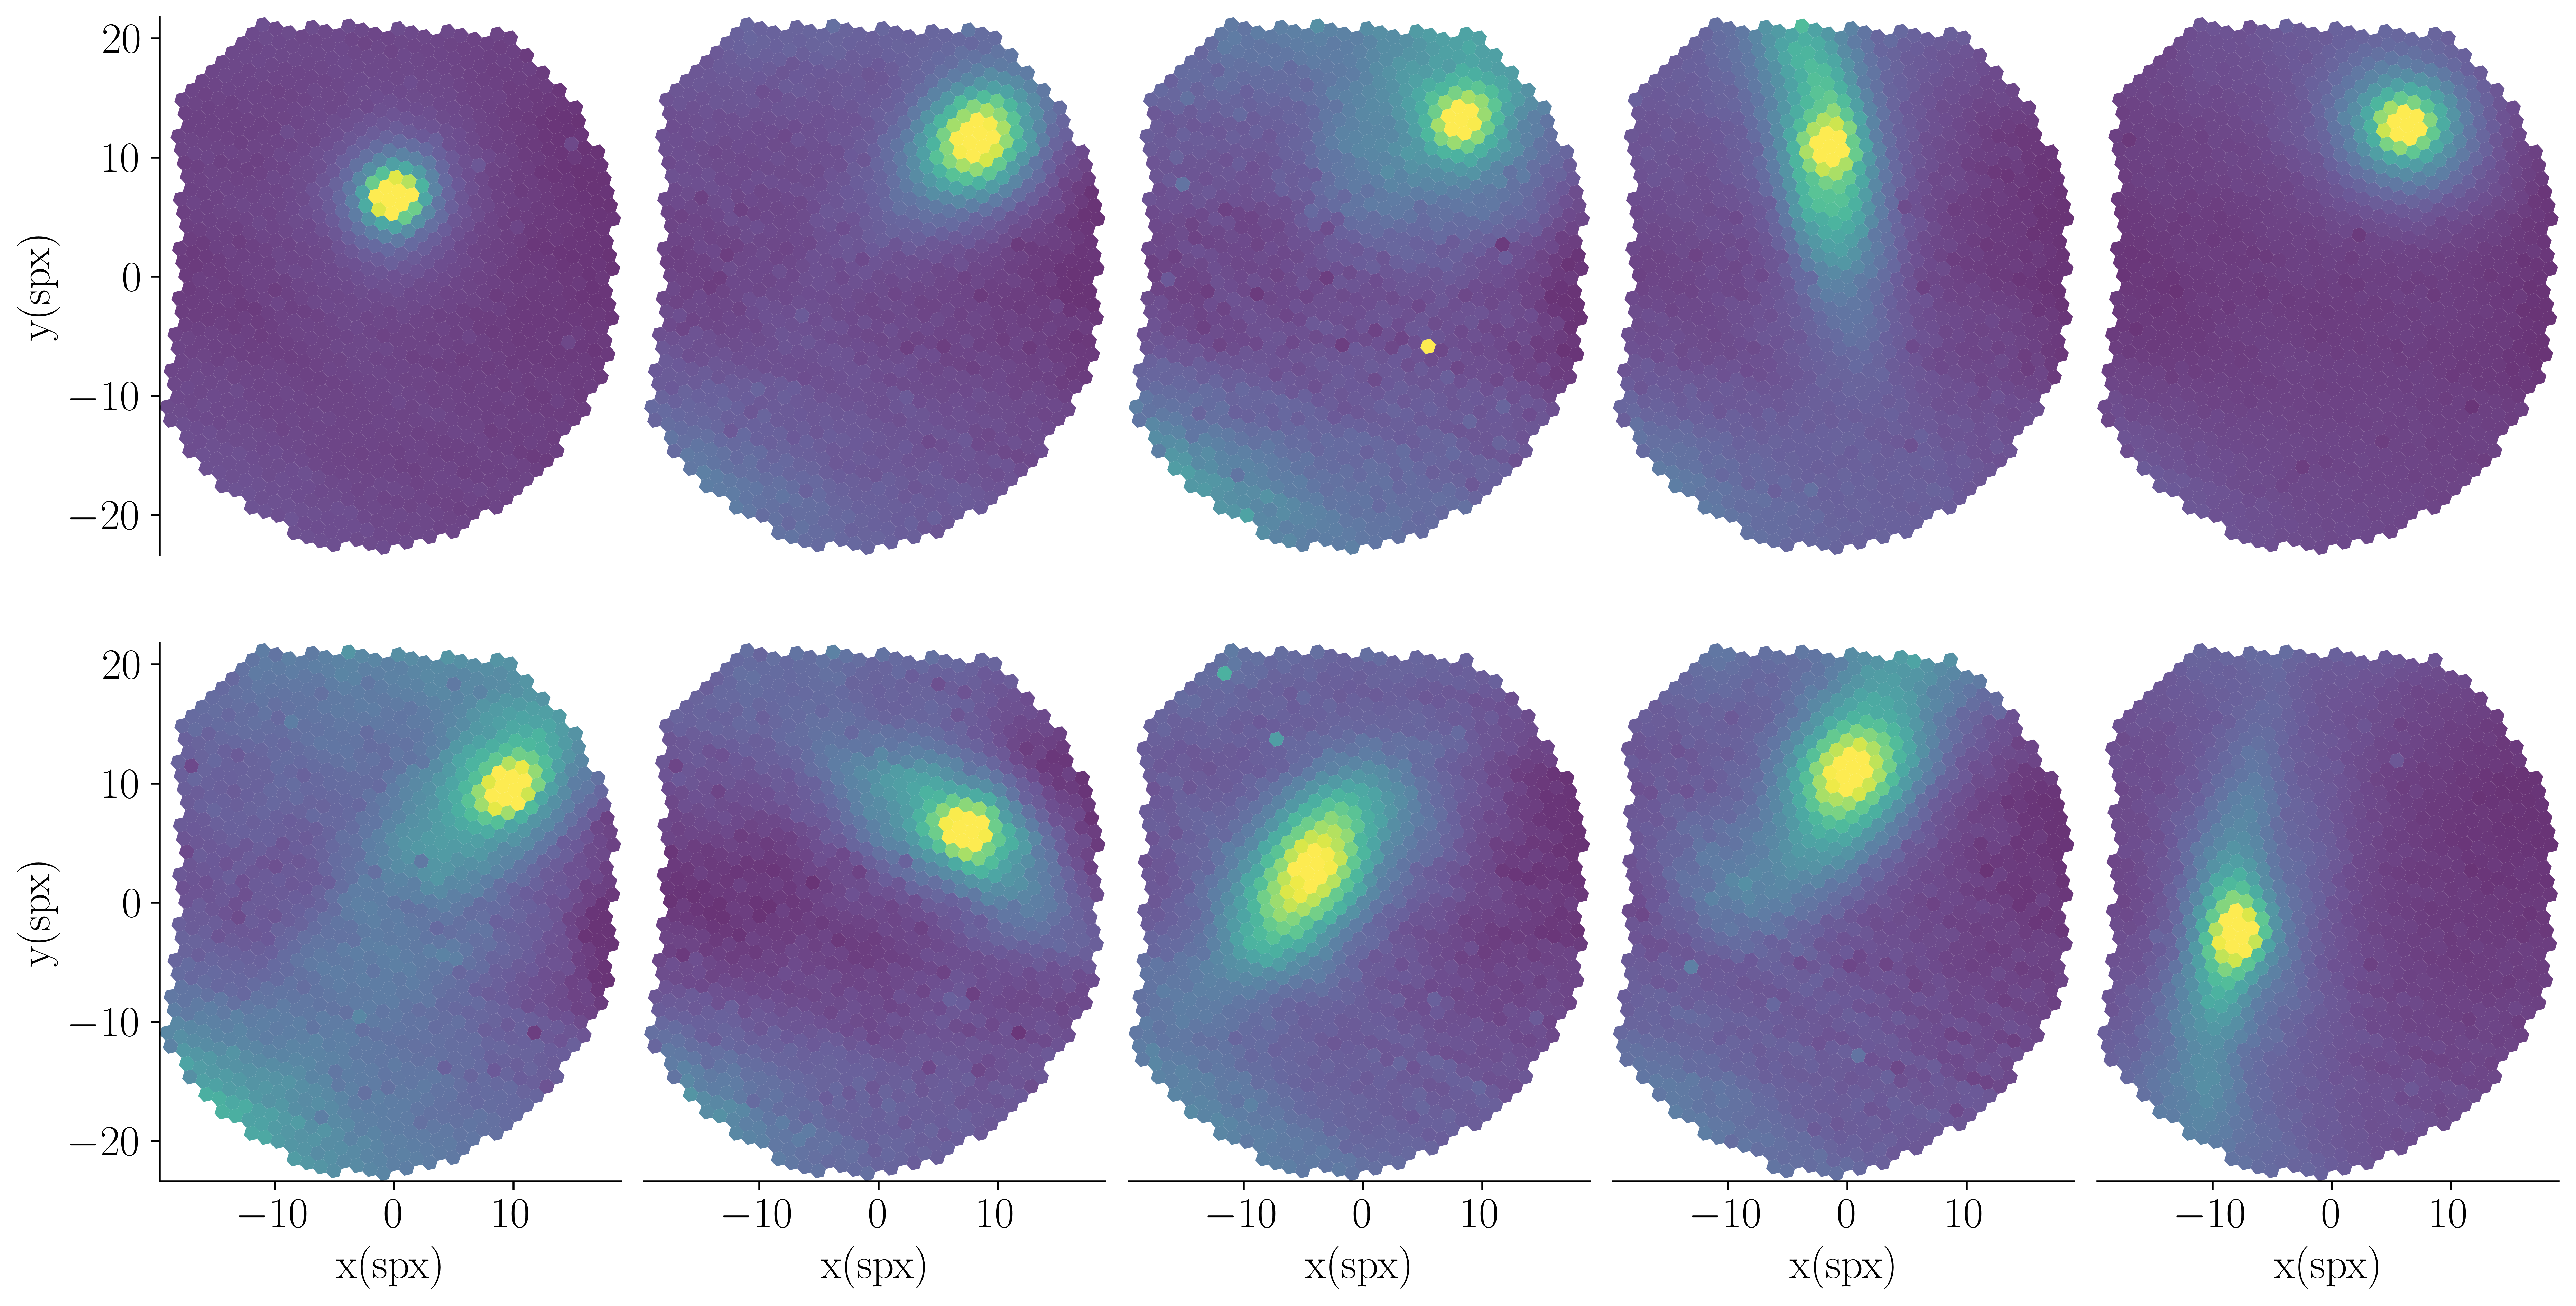
\includegraphics[width=0.99\textwidth]{../figures/08_simu/allhostsimu.pdf}
  \caption[Cubes de galaxies hôtes utilisés pour les simulations.]{Cubes
    intégrés (sur l'ensemble du domaine spectral de la SEDm) des galaxies hôtes utilisés pour les simulations. Bien que
    nous n'ayons pas eu l'opportunité d'avoir un grand nombre
    d'observations de galaxies isolées avec la SEDm, nous avons fait
    l'hypothèse que les morphologies et localisations variées de ces
    galaxies étaient suffisamment représentatives des observations pour
    constituer une base suffisante pour les simulations.}
  \label{fig:allhostsimu}
\end{figure}

\subsection{Spectres de supernovae}
% \label{ssec:xxx}

Afin de tester la précision d'extraction de spectre avec \hypergal, il nous faut inclure dans les cubes une source ponctuelle dont le
spectre est connu a priori. L'étude seule de la précision d'extraction
(par exemple avec un RMS spectral) est essentiellement indépendante de la forme du spectre, et donc du type
de la supernova.
Cependant nous souhaitons également avoir une
estimation de l'efficacité d'\hypergal\ à classifier les supernovae.
Pour analyser ces deux aspects (précision et classification), il faut
donc que le spectre de la source ponctuelle simulée soit connu a priori et que nous connaissions sa classification.

Afin de se rapprocher le plus possible des spectres observés par la SEDm, nous avons choisi
d'utiliser des spectres de supernovae déjà obtenus avec cet instrument, et
classifiés avec succès par \pkg{SNID}.

Afin de s'assurer de la classification, nous n'avons sélectionné que des
spectres avec un très haut r$lap$ (paramètre de qualité/confiance de SNID considéré
comme satisfaisant si r$lap>5$, voir section 6.1 de \citet{BlondinSNID}). Pour
les spectres de supernovae de type Ia (les plus nombreuses à être observées), nous avons
sélectionné $70$ spectres avec un r$lap>25$ pour le meilleur modèle, et un r$lap>15$ pour les 30 premiers modèles.

Sur un raisonnement similaire, nous avons sélectionné $7$ spectres de
supernova de type II avec un r$lap>12$. Pour les types Ic et Ib, plus
rarement observés ($\approx5\%$ des observations), nous avons
pris seulement $1$ spectre de chaque mais avec une forte
confiance de classification ( r$lap\approx22$ pour la Ib et r$lap\approx13$
pour la Ic).
Chacun de ces spectre est ensuite lissé par application d'un filtre de Savitzky-Golay \citep{SavitzkyGolay}. Afin de ne pas casser les
structures des spectres, nous utilisons un lissage léger avec un
polynôme d'ordre 3 sur une fenêtre de 5 pixels spectraux.

Nous montrons dans la Figure~\ref{fig:specsimueach} quelques exemples de
spectre après lissage pour chaque type de supernova, ainsi que le
meilleur modèle de classification SNID et le r$lap$ associé.

\begin{figure}[ht]
  \centering
  \includegraphics[width=0.9\textwidth]{../figures/08_simu/specsimueach.pdf}
  \caption[Exemple de spectres pour chaque type de supernova pour les
  simulations.]{Exemple de quelques spectre pour chaque type de supernova pour
    les simulations. Nous y montrons en gris le spectre utilisé pour les
    simulations qui provient d'une
    observation de la SEDm, et en couleur le meilleur
  modèle de classification SNID avec le r$lap$, redshift et phase associés.}
  \label{fig:specsimueach}
\end{figure}
\clearpage
\subsection{\'Echantillon d'étude}
% \label{ssec:xxx}

\subsubsection{Types et phases}

Dans le but de représenter dans nos simulations les proportions
observées de chaque
type de supernova, nous utilisons les statistiques de la Data
Release 1 du groupe Bright Transient Survey de ZTF
\citep[BTS;][]{FremlingZTFspec2020}.
Nous choisissons ainsi de répartir dans nos simulations $80\%$ de SNeIa,
$15\%$ de SNeII, $2.5\%$ de SNeIb et $2.5\%$ de SNeIc. Ces deux derniers
types sont habituellement regroupés, nous considèrerons donc par la
suite un groupe de $5\%$ de SNeIbc.

Nous choisissons également de 
procéder à une marginalisation des phases des spectres de SNeIa, en se
basant sur les statistiques de la
DR1 du groupe SNeIa de ZTF \citep{DhawanZTFDR1}. Pour
les 70 spectres utilisés, nous déduisons la phase en comparant le
jour d'observation de la supernova avec le pic
de luminosité ajusté par ZTF avec SALT2
\citep{Guysalt2005,Guysalt22007,Guy2010,Betoule2014} sur la courbe de
lumière.

La distribution de phase de notre échantillon s'étend de -15 à
+15 jours, avec une médiane à -2 jours. Nous pouvons ainsi sélectionner
aléatoirement les spectres de SNIa, sachant leur phase et suivant une
distribution équivalente à celle relevée dans \citet{DhawanZTFDR1}. Nous marginalisons nos simulations suivant
une distribution de phase gaussienne, centrée sur $-3$ jours et d'écart
type $4$ jours.

\subsubsection{Seeing}

Les supernovae étant des sources ponctuelles à ajouter dans nos cubes
de simulations, elles sont entièrement caractérisées par leur profil de
PSF.

Nous utilisons le profil radial développé au chapitre~\ref{ch:irf} avec
l'étude des étoiles standards. Afin de représenter une distribution en
seeing similaire à celle observée par la SEDm, nous marginalisons nos
simulations sur le seeing en utilisant les
distributions conjointes des paramètres de forme de PSF ajustés des $2202$
étoiles standards extraites pour l'étude de la calibration en
flux (section~\ref{sec:validationpsf}). Le profil de PSF chromatique est
entièrement défini par $3$ paramètres de forme: $\alpha_{ref}$, $\eta$ et $\rho$,
où $\alpha_{ref}$ correspond à la largeur de la Moffat à une longueur
d'onde de référence $\lambda_{ref}$ arbitraire, que nous fixons à $6000$ \AA.

Nous faisons donc la supposition que la distribution en seeing des
étoiles standards est représentative de celle des supernovae. Bien que
la contribution de l'optique du télescope soit indépendante
de l'objet observé, il faut noter que les étoiles standards le sont
habituellement avec une masse d'air comprise entre $1$ et
$1.2$. Nos simulations ayant une masse d'air comprise entre $1$ et $2$, cela implique potentiellement une sous-estimation de la
distribution en seeing utilisée pour nos simulations que nous
n'avons pas caractérisé. Nous montrons dans la
Figure~\ref{fig:psfparams} les distributions conjointes des paramètres
de forme de PSF utilisés pour les simulations. 

\begin{figure}[ht]
  \centering
  \includegraphics[width=0.99\textwidth]{../figures/08_simu/simupsfparams_corner.pdf}
  \caption[Distribution conjointe des paramètres de PSF des
  simulations.]{Distribution conjointe des paramètres de PSF utilisés
    pour les simulations. Le niveau de gris indique la densité de simulations
  dans un intervalle donné.}
\label{fig:psfparams}
\end{figure}

La Figure~\ref{fig:simufwhm} correspond à la distribution en seeing
sous-jacente, avec une médiane de $1\farcs67$, très proche de la valeur
indiquée dans \citet{SEDM18} de $1\farcs68$.

\begin{figure}[ht]
  \centering
  \includegraphics[width=0.9\textwidth]{../figures/08_simu/simupsf_fwhm.pdf}
  \caption[Distribution du seeing des simulations.]{Distribution
    du seeing pour les simulations en arcsec.}
\label{fig:simufwhm}
\end{figure}


\subsubsection{Distance supernova/centre galactique}\label{ssec:distancesimu}

\hypergal\ a été conçu pour répondre à la problématique de la
contamination de la source ponctuelle par la galaxie hôte. Nous voulons donc explorer la
précision d'extraction de spectre des SNe et l'efficacité de
classification suivant la distance séparant la source ponctuelle du
centre galactique. Dans ces simulations nous ne nous intéressons pas aux
cas où la supernova est complètement isolée dans le champ de vue,
puisque la contribution de la galaxie est alors marginale et
la méthode d'extraction devient identique à celle des étoiles standards.

Nous utilisons une distribution uniforme comprise entre $0$ et $10$
spaxels de distance, ce qui correspond à un écart maximal de
$\approx5\farcs6$. Cette distance seuil représente environ $2$ à $3$ largeur à
mi-hauteur suivant le profil radial des sources ponctuelles, ce qui nous
semble suffisant pour explorer un large intervalle de séparation
angulaire jusqu'à la limite d'un fond non structuré. 

Nous prenons également en compte que lors des observations réelles, les
supernovae sont habituellements situées vers le centre du MLA. Ainsi
afin d'éviter de simuler une cible dans un des coins du cube, nous
restreignons la localisation possible de la source ponctuelle dans un
cylindre de $12$ spaxels de rayon au centre du MLA. Pour les cas où la
galaxie est très excentrée et que nous simulons une source ponctuelle
proche du centre galactique, nous privilégions de la positionner dans le
quart de cercle en direction du centre du MLA. 

\subsubsection{Constraste}

Le dernier paramètre que nous utilisons pour explorer la robustesse
d'\hypergal\ correspond à l'intensité du flux de la supernova par
rapport au signal de fond: nous introduisons ainsi le
contraste $c_{r}$, défini dans la bande photométrique équivalente $r_{\text{ZTF}}$
afin de pouvoir plus aisément comparer les résultats des simulations
avec un cas réel d'observation. Nous exprimons ce paramètre de la façon suivante:
\begin{equation}
  \label{eq:contrast}
  c_{r} = \frac{S_{r}}{S_{r}+B_{r}}
\end{equation}
avec $S_{r}$ le signal de la supernova et $B_{r}$ le signal de tout ce qui se
situe en fond (ciel + galaxie), tout deux intégrés dans la bande
équivalente $r$.

Afin de déterminer la quantité $B_{r}$ qui contamine le signal de la
supernova, nous prenons en compte le profil de PSF utilisé pour
simuler la source ponctuelle.
Plutôt que de considérer une ouverture fixe
autour de la localisation de la SN simulée pour définir $B_{r}$, nous
multiplions le cube de simulation sans la SN par un cube ne contenant
que le profil de PSF (normalisé avec un pic à $1$) à la localisation de
simulation de la SN. En faisant cela nous pondérons spatiallement le
signal de contamination $B_{r}$ par le profil de PSF simulé de la SN.

Le contraste est défini dans l'intervalle $[0,1]$, $0$ impliquant
que la supernova n'existe pas, et $1$ qu'elle est infiniment plus
intense que le fond (ou que le fond est à zéro ce qui n'est pas notre
cas ici).

La Figure~\ref{fig:host_contrast_simu} illustre l'uniformité de la
distribution en contraste et de la distribution en distance SN-centre
galactique.

\begin{figure}[ht]
  \centering
  \includegraphics[width=0.99\textwidth]{../figures/08_simu/simu_host_contrast.pdf}
  \caption[Distribution du contraste et de la distance SN-centre de la
  galaxie des simulations.]{Distribution du contraste et de la distance SN-centre de la
  galaxie des simulations}
\label{fig:host_contrast_simu}
\end{figure}

\begin{comment}
Nous pouvons également relier le contraste au rapport $R=\frac{S_{r}}{B_{r}}$:
\begin{equation}
  \label{eq:rapportSB}
  c_{r} = \frac{R}{1+R}
\end{equation}

Les simulations sont ainsi générées suivant une distribution uniforme du
contraste $c_{r}$ entre $0$ et $1$.

Nous pouvons également voir que le rapport signal sur bruit est
étroitement lié au contraste. En effet, en supposant que le signal dans
le cube est
entièrement caractérisée par une loi de Poisson, nous avons alors que:

\begin{equation}
  \label{eq:SNR}
  SNR_{r} \triangleq \frac{S_{r}}{\sqrt{\sigma_{S_{r}}^{2}+\sigma_{B_{r}}^{2}}}\approx
  \frac{S_{r}}{\sqrt{S_{r}+B_{r}}} = c_{r}\times\sqrt{S_{r}+B_{r}}
\end{equation}
avec $S_{r}$ et $B_{r}$ en unités de coups. Avec un raisonnement similaire nous
pouvons montrer que:
\begin{equation}
  \label{eq:logsnr}
  SNR_{r}\approx R\times\sqrt{B_{r}} = \frac{C_{r}}{1-C_{r}}\times\sqrt{B_{r}}
\end{equation} 

En pratique, nous sommes en mesure de récupérer la quantité
$\sigma_{B}$, car présente dans le cube SEDm avec la galaxie hôte
isolée. Pour remonter au SNR, nous utilisons directement sa définition
en supposant que le bruit à ajouter dans le cube à cause du signal de la
supernova simulée est $\sigma_{S}^{2}=S$.
\end{comment}
\subsection{Création des cubes de simulation}

Après avoir procéder à la marginalisation des proportions de chaque type
de supernova, de la phase des Ia et du seeing, nous générons un jeu de
$N\times m$ paramètres avec $N$ le nombre de simulations (5000), et $m$
les paramètres de la simulation:\\

\begin{itemize}[label=$\diamondsuit$]
  \itemsep0em
 \begin{samepage}
\item Cube de la galaxie hôte ($i=1,2..,n$);
\item Spectre de supernova (type, phase);
\item Paramètres de PSF décrivant la SN ($\alpha$, $\eta$, $\rho$);
\item Distance entre la SN et le centre galactique ($d$);
\item  Contraste ($c_{r}$).
  \end{samepage}
\end{itemize}

Connaissant \textit{a priori} la calibration en flux utilisée pour chacun des
cubes, nous appliquons une calibration inverse sur le spectre de la SN à simuler,
qui est initialement en unité de flux physique.
Cela nous permet de traailler en ADU, et ainsi d'ajouter le signal de la supernova simulée et le
bruit associé.

La création d'un cube de simulation sachant les $m$ paramètres se fait ensuite en plusieurs étapes:

%\begin{minipage}{\textwidth}%
  \begin{enumerate}[(a)]
    \itemsep=0em
    \item \textbf{Détermination de la localisation ($x_{ref}$, $y_{ref}$) de la supernova} dans le cube
      à une longueur d'onde de référence ($\lambda_{ref}=6000$\AA):
      nous prenons aléatoirement une position sur le cercle centré sur
      la galaxie, avec un rayon égal à la distance choisie
      SN-galaxie. Nous prenons en compte les contraintes pour éviter les
      bords du cube expliquées dans la section~\ref{ssec:distancesimu};
      
  \item \textbf{Détermination du signal de fond $B_{r}$:} nous construisons un cube vide dans
    lequel nous plaçons le profil de PSF à la localisation et longueur
    d'onde fixée à l'étape
    précédente. Le pic du profil est normalisé à 1. Nous appliquons les
    effets d'ADR (déviation chromatique du centroïde), sachant les paramètres de masse d'air et
    d'angle parallactique effectif de la galaxie. Nous multiplions alors
    le cube de la galaxie par
    ce cube ne contenant que le profil de PSF simulé dont le pic est
    normalisé à 1, le résultat étant un nouveau cube contenant uniquement le signal de fond $B$
    contaminant la SN. Connaissant la transmission du filtre $r$ de ZTF,
    nous déterminons $B_{r}$.

  \item \textbf{Détermination du coefficient multiplicatif à appliquer sur le
    spectre de la supernova.} Connaissant le spectre de la
    supernova en ADU, nous en déduisons son signal $\tilde{S}_{r}$ dans
    la bande $R$ avant adaptation au
    contraste souhaité. Sachant $B_{r}$, $\tilde{S}_{r}$ et le contraste
    $c_{r}$, nous
    appliquons le
    coefficient multiplicatif nécessaire sur l'ensemble du spectre de la
    SN (et donc sur $\tilde{S}_{r}$) pour obtenir le constraste
    souhaité. Le spectre final est noté $S$, et l'intégration dans la
    bande équivalent $r$ correspond à $S_{r}$.

   \item \textbf{Ajout du bruit associé à la supernova.} Nous supposons que le
     flux ajouté de la supernova simulée génère un bruit entièrement caractérisé
     par une loi de Poisson. Nous ajoutons donc au cube SEDm pour chaque
     spaxel de chaque tranche une variance telle que
     $\sigma_{S}^{2}=S$.

   \item \textbf{Détermination du SNR.} Le SNR n'est pas un paramètre de
     nos simulations, mais nous pouvons l'estimer connaissant
     $S_{r}$, $\sigma_{B_{r}}$ et  $\sigma_{S_{r}}$. On définit le SNR
     dans la bande $r$ comme
     $\text{SNR}_{r}=\frac{S_{r}}{\sqrt{\sigma_{B_{r}}^{2}+\sigma_{S_{r}}^{2}}}$,
     où $\sigma_{B_{r}}$ est naturellement présent dans le cube de la
     galaxie et contient les contributions de la galaxie, du ciel et du
     bruit de lecture. $\sigma_{S_{r}}$ est déterminé à l'étape précédente.

   \item \textbf{Construction du cube de simulation}. Tous les
     ingrédients sont réunis pour la construction du cube: le spectre de
     la supernova, sa position chromatique, son profil de PSF
     chromatique et le coefficient multiplicatif pour avoir le contraste désiré.
  \end{enumerate}
%\end{minipage}\\


Nous procédons ainsi à la générations des $5000$ cubes de
simulations. Dans la Figure~\ref{fig:examplesimu} nous illustrons
quelques exemples de ces cubes pour différentes valeurs de contraste,
distance, type de SN et SNR.
\begin{figure}[ht]
  \centering
  \makebox[\textwidth][c]{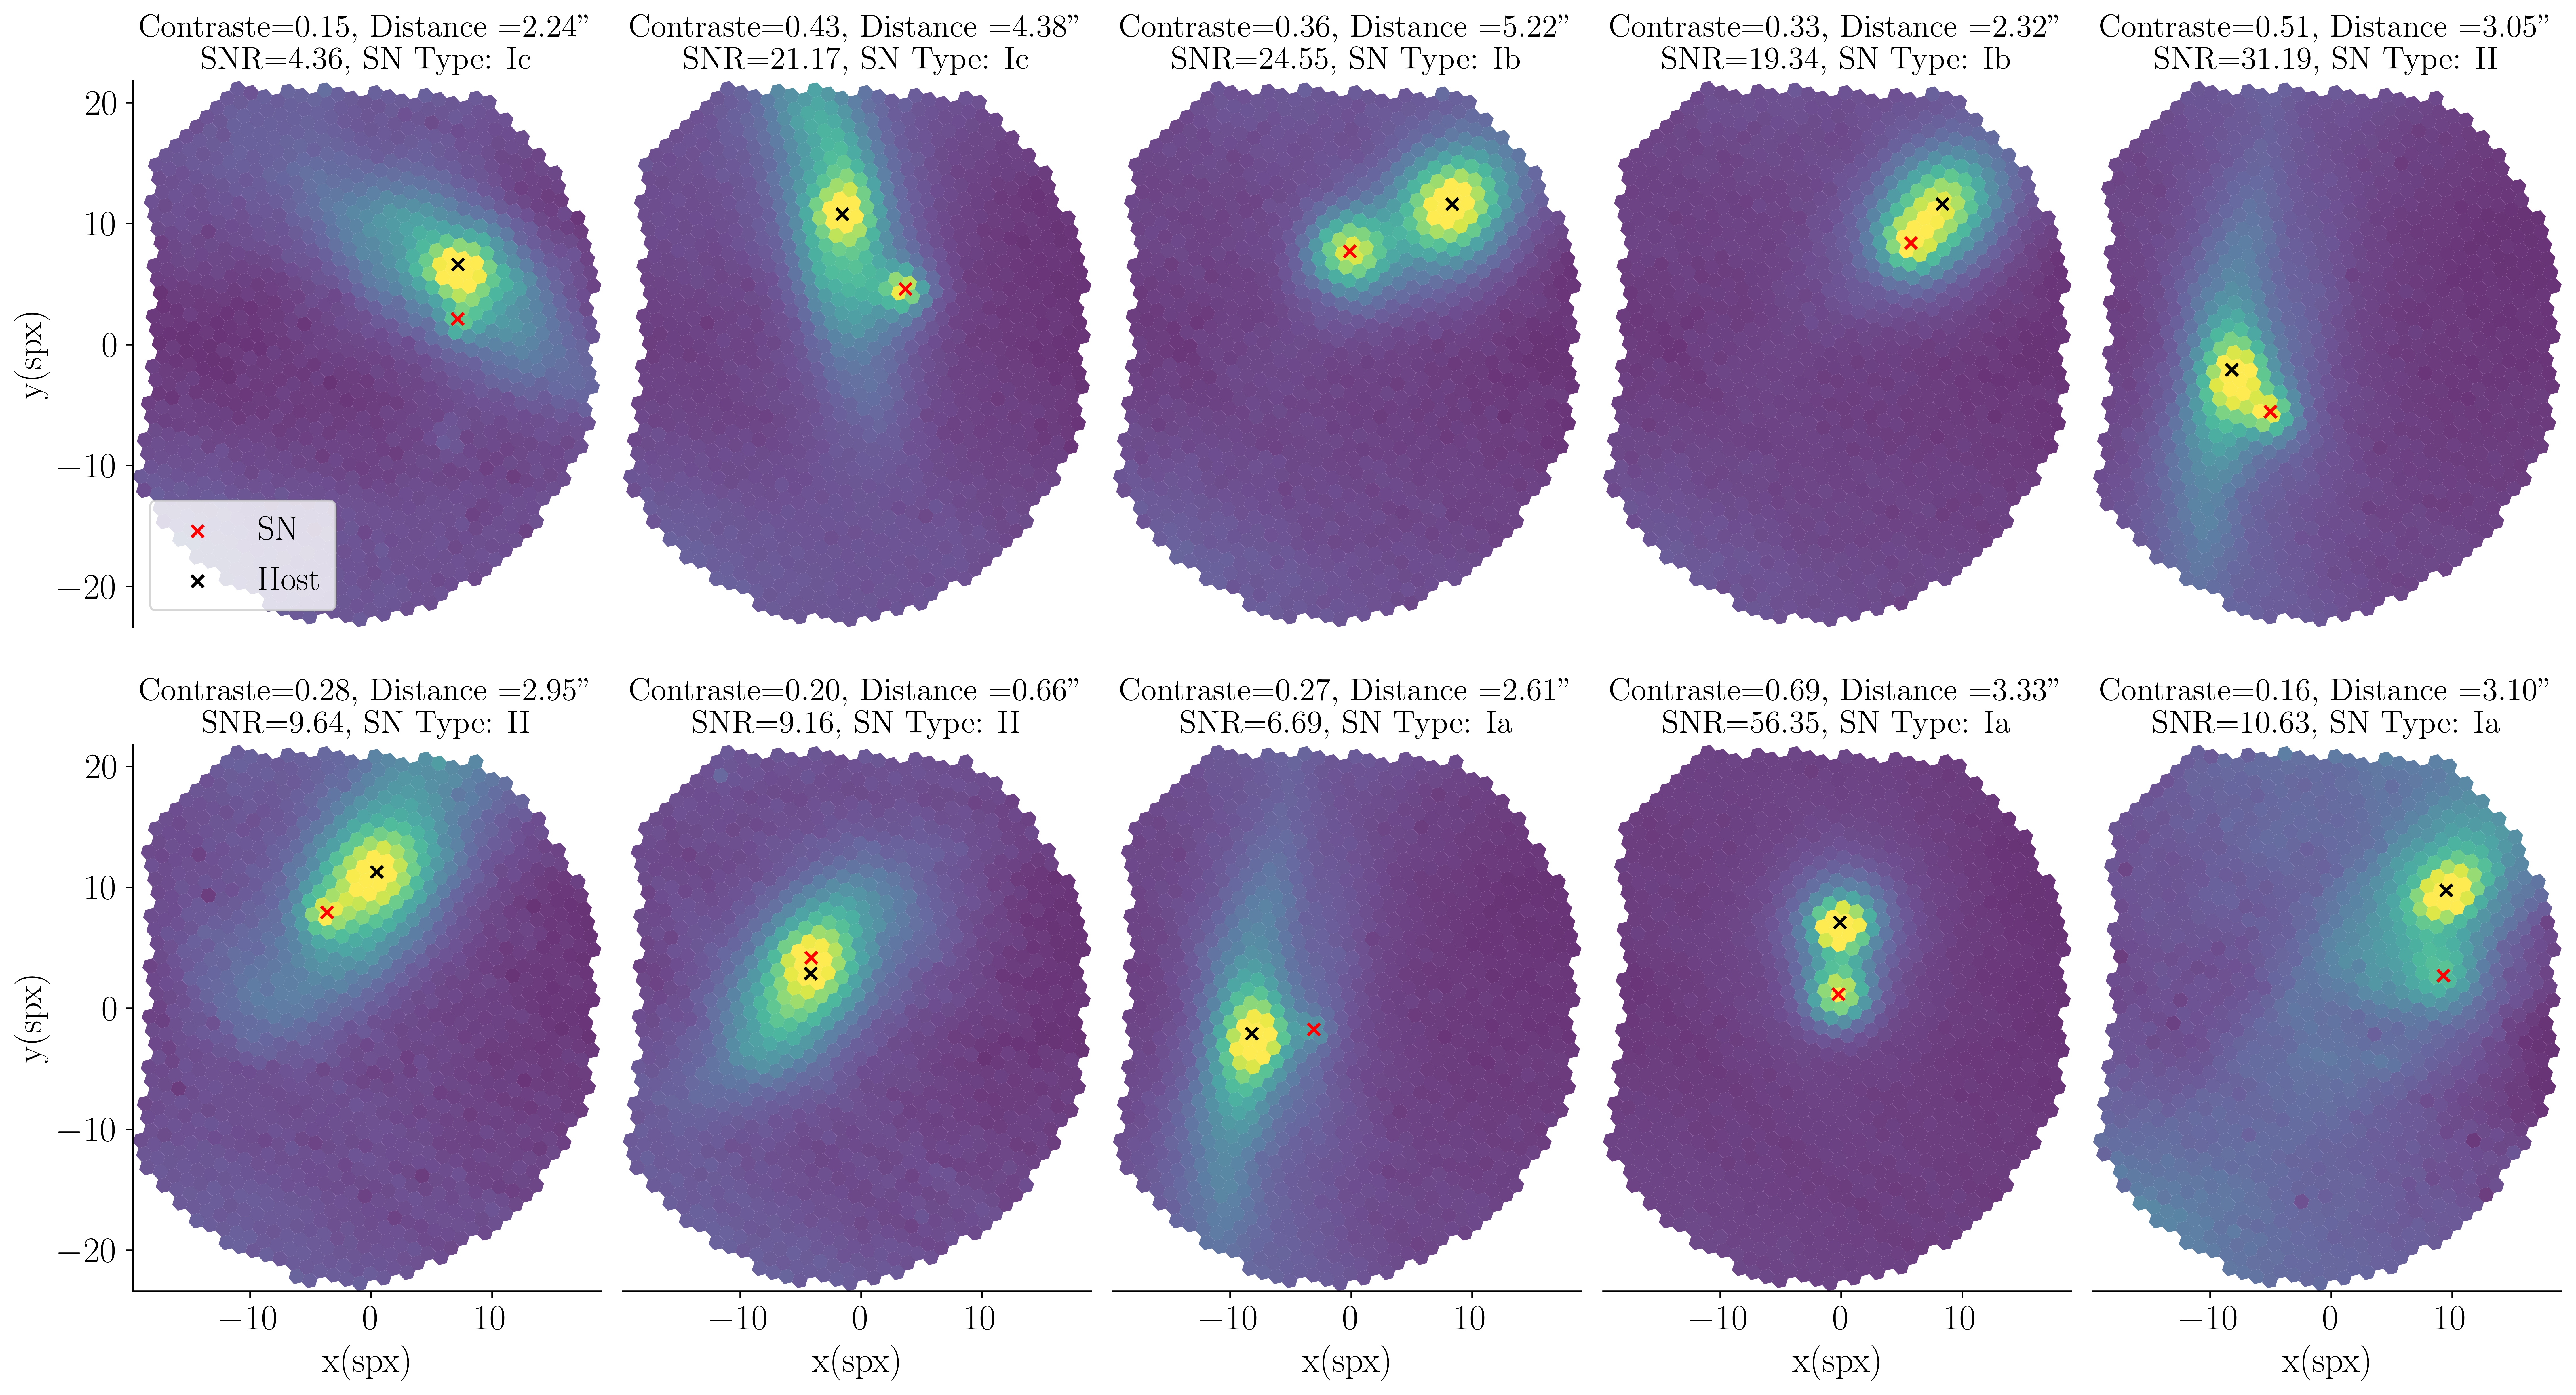
\includegraphics[width=1.15\textwidth]{../figures/08_simu/examplesimu.pdf}}%
  \caption[Examples de cubes de simulation.]{Examples de cubes de
    simulation pour différentes valeurs de contraste, distance, type de
    SN et SNR.}
  \label{fig:examplesimu}
\end{figure}

\section{Résultats et précision}\label{sec:simuresult}

Après avoir généré nos cubes de simulation, nous avons fait tourner
\hypergal\ suivant 2 méthodes: la première avec une modélisation de
scène complète comprenant toutes les composantes comme détaillée au chapitre
précédent. Puis une deuxième fois avec la méthode d'extraction similaire au
pipeline d'origine \pysedm, sans modélisation de la galaxie hôte,
utilisé comme référence.

Nous n'avons pas utilisé directement le pipeline \pysedm\ car les modèles
de PSF et de fond sont différents de celui d'\hypergal, ce qui n'aurait
pas permis une comparaison juste. La méthode d'extraction est cela dit
identique, suivant le procédé détaillé dans \citet{pysedm} et la section~\ref{ssec:sourceextractpysedm}.
Les seules différences avec la modélisation de scène complète sont
l'absence de modèle de galaxie et le fait que l'on ne considère qu'un
disque de $10$ spaxels de rayon autour de la position de la supernova
pour son extraction.

En plus d'une étude de la robustesse absolue d'\hypergal, cette
confrontation nous permet d'avoir également une idée de l'amélioration
apportée avec ce nouvel outil d'extraction de spectre.

Nous dénominerons dans la suite du manuscrit l'indice $_{HG}$ pour la
méthode de modélisation de scène \hypergal, et $_{PS}$ pour la méthode
d'extraction de source ponctuelle basique.

Dans cette section nous allons étudier 3 informations pour chacune des 2
méthodes:

\begin{itemize}[label=$\diamondsuit$]
  \itemsep0em
 \begin{samepage}
\item \textbf{La précision spectrophotométrique}, c'est à dire une
  comparaison directe du spectre d'entrée de simulation et du spectre extrait;
\item \textbf{La précision après correction du continuum}, à l'instar de
  la méthode de pré-traitement utilisé par le classifieur \pkg{SNID}
  (section~\ref{sec:snid}). La SEDm ayant été conçu pour la
  classification de spectres, ce qui nous importe est la
  capacité d'\hypergal\ à extraire les informations spectrales
  permettant cette classification, c'est à dire les structures spectrales
  traduisant les caractéristiques de tel ou tel type. Nous nous
  affranchissons ainsi d'éventuels problèmes de calibrations absolues et
  relatives au flux.
\item \textbf{L'efficacité de classification}. Pour cela nous
  utiliserons le même classifieur utilisé par ZTF, \pkg{SNID}, et nous
  comparerons la classification du spectre extrait avec celui connu a priori.
  \end{samepage}
\end{itemize}


\begin{comment}
Plutôt que d'utiliser le contraste comme paramètre d'étude, nous
utiliserons le rapport signal sur bruit. Comme introduit dans
l'équation~\ref{eq:logsnr}, le SNR est étroitement lié au
contraste car linéairement proportionnel au rapport $R=S_{r}/B_{r}$. Nous illustrons cette corrélation dans la
Figure~\ref{fig:corr_SNR_contrast}, montrons la relation linéaire entre
le SNR et la quantité $R=\frac{C_{r}}{1-C_{r}}$.

\begin{figure}[ht]
  \centering
  \makebox[\textwidth][c]{\includegraphics[width=1.\textwidth]{../figures/08_simu/corr_SNR_contrast.pdf}}%
  \caption[Corrélation SNR/contraste des simulations.]{Corrélation
    SNR/contraste des simulations et leur distribution respective. Nous
    montrons dans cette figure en échelle logarithmique le rapport signal
    sur bruit en fonction de la quantité $R=\frac{C_{r}}{1-C_{r}}$,
    introduite dans l'équation~\ref{eq:logsnr}. La
    droite en pointillés rouge indique la régression
    linéaire, et la dispersion autour de celle ci provient de la
    contribution du fond, $\sqrt{B_{r}}$, propre à chaque simulation.}
  \label{fig:corr_SNR_contrast}
\end{figure}

\end{comment}
\subsection{Précision spectrophotométrique}\label{ssec:spectrophotoaccuracy}

Commençons par étudier la capacité d'extraction spectrophotométrique d'\hypergal\ et de la méthode
d'extraction simple. Pour ce faire nous calculons pour chaque simulation
le RMS spectral, dans l'intervalle de longueur d'onde utile à la
classification, c'est à dire [$4000$,$8000$] \AA. Nous regardons ensuite
l'évolution de ce RMS en fonction du contraste et de la distance
angulaire entre la SN et le centre de la galaxie.

Dans un premier temps, nous avons vérifié les corrélations entre la
distribution des RMS calculés des deux méthodes et les différents
paramètres de la simulation
(Figure~\ref{fig:corrheatmap_simuparams_spectrophoto}). Nous remarquons
sans surprise
que la précision d'extraction est fortement corrélée ($\rho=-0.83$) avec
le contraste, mais très peu ($\rho=-0.16$) avec la distance séparant la SN de la
galaxie. Cette contribution est cependant plus
élevée ($\rho=-0.33$) pour la méthode classique d'extraction, attestant
qu'à proximité de la galaxie l'approximation de fond non structuré n'est
plus correcte, et dégrade l'extraction.

\begin{figure}[ht]
  
  \includegraphics[width=\textwidth]{../figures/08_simu/corrheatmap_simu_params_spectrophoto.pdf}
    \caption[Corrélation des paramètres de la
    simulation (spectrophotométrique).]{Carte des coefficients de corrélation de Pearson des
      paramètres principaux de la
    simulation dans l'étude spectrophotométrique. \emph{À gauche} les
    corrélations pour la modélisation de scène complète. La corrélation
    entre la distance SN-centre de la galaxie et
    le RMS spectre d'entrée-spectre de sortie est quasiment inexistante pour la méthode
    \hypergal. \emph{À droite} nous montrons les mêmes corrélations pour
    la méthode d'extraction de référence, sans modélisation
    hyperspectrale de la galaxie. Bien que modérée, la
    distance montre une plus forte corrélation avec le RMS pour cette méthode.}\label{fig:corrheatmap_simuparams_spectrophoto}
\end{figure}


Passons maintenant à l'analyse de la distribution du RMS spectral.
La Figure~\ref{fig:simu_rms_snr_spectrophoto} illustre l'évolution du
RMS spectral en fonction du contraste, en considérant des intervalles
linéaires contenant la même quantité de simulations.
La première information ressortant clairement de ces résultats est
l'amélioration indiscutable obtenue avec la modélisation hyperspectrale
de la galaxie, quelque soit le contraste. Par ailleurs, la méthode d'extraction basique
semble clairement inutilisable spectrophotométriquement sur l'ensemble
de la simulation, ne descendant sous les $10\%$ de RMS qu'à partir d'un
contraste $c\approx0.8$.

La modélisation de scène quant à elle
approche un RMS$\approx10\%$ à partir d'un contraste $c\approx0.5$, et
descend sous les $5\%$ vers un $c\approx0.7$. 

Nous montrons également la distribution des 3 permiers quartiles du
rapport $\frac{RMS_{HG}}{RMS_{PS}}$, et nous pouvons visualiser une
amélioration significative (d'un facteur $2$ minimum pour $75\%$ des simulations) entre les deux
méthodes quelque soit l'intervalle de contraste considéré. 

\begin{figure}[ht]
  \centering
  \makebox[\textwidth][c]{\includegraphics[width=0.9\textwidth]{../figures/08_simu/simu_rms_contrast_spectrophoto.png}}%
  \caption[Distribution du RMS spectral en fonction du
  SNR.]{Distribution du RMS spectral entre le spectre d'entrée de la
    simulation et le spectre extrait en fonction du SNR  sur l'intervalle [$4000$,$8000$]\AA. Les
    distributions sont présentées en boîtes, dont les 3 barres
    centrales représentent les 3 quartiles ($25\%$, médiane et $50\%$). Nous illustrons ici une
    distribution de RMS spectral pour chacune des deux méthodes
    d'extraction et pour différents intervalles de contraste, chacun comptabilisant le
    même nombre de simulation. Nous montrons \emph{en haut} le RMS
    spectral (en $\%$) obtenu avec les deux méthodes 
    en fonction du contraste. Les traits en pointillés indiquent les niveaux à
    $1\%$, $5\%$ et $10\%$. \emph{En bas} nous montrons le rapport
    $\frac{RMS_{HG}}{RMS_{PS}}$ pour illustrer l'amélioration apportée par
    \hypergal. Nous ne montrons que la boîte représentant les 3 quartiles de
    chaque distribution pour plus de clareté visuelle.}
  \label{fig:simu_rms_snr_spectrophoto}
\end{figure}

Cette différence de précision entre les deux méthodes, quelque soit le
contraste, s'explique par l'influence de la distance pour l'extraction
de référence. Contrairement à \hypergal\, le spectre extrait sera
systématiquement plus dégradé si la SN ne se distingue pas suffisamment
de la galaxie, où l'approximation d'un fond linéaire est justifiée.
Nous illustrons cela dans la
Figure~\ref{fig:simu_rms_dist_spectrophoto}, où nous présentons la même
analyse mais en fonction d'intervalles de distance apparente entre la
galaxie hôte et la supernova. Aucune corrélation avec la
distance n'est visible pour la modélisation de scène complète comme
explicité par la matrice de corrélation. La méthode d'extraction simple en revanche montre une
forte dégradation lorsque la distance est inférieure à
$4\arcsec$. Ce sont les contributions des extractions sous ce seuil qui
traduisent la surperformance d'\hypergal\ lorsque l'on ne
considère que le contraste et que l'on marginalise sur la distance.

\begin{figure}[ht]
  \centering
  \makebox[\textwidth][c]{\includegraphics[width=0.9\textwidth]{../figures/08_simu/simu_rms_dist_spectrophoto.png}}%
  \caption[Distribution du RMS spectral en fonction de la distance
  hôte/SN.]{Même chose que pour la
    Figure~\ref{fig:simu_rms_snr_spectrophoto} mais en fonction de la distance.}
  \label{fig:simu_rms_dist_spectrophoto}
\end{figure}

Quelque soit l'angle d'étude de la précision d'extraction spectrophotométrique,
la méthode incluant la modélisation hyperspectrale de la galaxie hôte
démontre une nette amélioration en comparaison avec une extraction
basique comme celle proposée par \pysedm.

Nous observons cependant que même le RMS spectral obtenu avec \hypergal\
ne permet pas d'étude scientifique
spectrophotométrique avec la SEDm, à moins que le contraste soit
suffisamment élevé.
Cet instrument, tout comme ce pipeline, ne sont heureusement pas conçus à
cet effet mais à la classification des supernovae observées.

La classification utilise la structure du spectre au travers des raies
d'absorptions/émissions caractéristiques de l'objet observé. La
classification va donc se baser sur les corrélations entre le spectre
extrait et une base de modèle dont la classification est a priori
connue. En ce sens, nous avons choisi d'analyser le RMS spectral en
retirant le continuum des spectres extraits, à l'instar de ce qui est
effectué par \pkg{SNID} \citep{BlondinSNID}.


\subsection{Précision avec correction de continuum}
% \label{ssec:xxx}

Afin de faire en sorte que le RMS spectral sonde les structures spectrales
plutôt que le flux total ou la couleur, nous divisons les deux spectres par leur continuum
respectif. Bien que \pkg{SNID} utilise un polynome 
d'ordre $13$ pour déterminer ce continuum, nous préférons procéder à
cet ajustement avec un polynome
d'ordre $5$ afin d'éviter un potentiel sur-ajustement de certaines
caractéristiques des spectres.

Nous illustrons cette correction dans la
Figure~\ref{fig:continuumcorrection_ex}, où nous montrons la comparaison
entre un spectre extrait et celui simulé, avant et après division du
continuum. Nous pouvons visualiser dans cet exemple un effet de couleur
lors de l'extraction menant à un RMS spectral spectrophotométrique de
plus de $33\%$. La distance entre la SN et le centre de la galaxie dans
cet exemple est de seulement $0\farcs86$, soit moins de deux
spaxels. En corrigeant par le continuum, on remarque que toutes
les structures du spectres sont nettement extraites par \hypergal, et
le RMS spectral tombe à $6\%$.

\begin{figure}[ht]
  \centering
  \makebox[\textwidth][c]{\includegraphics[width=1.2\textwidth]{../figures/08_simu/continuumcorrection_ex.png}}%
  \caption[Exemple de RMS spectral pour une simulation après correction
  du continuum.]{Exemple de RMS spectral après
    correction du continuum (contraste de $0.27$
    et une distance hôte/SN de $0\farcs86$). \emph{À gauche} la comparaison du spectre simulé (en bleu) et du spectre
    extrait par \hypergal\ (en rouge), ainsi que le rapport entre les
    flux. On observe un effet de
    couleur dégradant fortement le RMS spectrophotométrique sur
    l'intervalle [$4000$,$8000$]\AA, atteignant plus de $33\%$. Les
    courbes en pointillés représentent le continuum ajusté avec un
    polynome d'ordre $5$. \emph{À droite} sont présentés les mêmes
    spectres après division par le continuum. La
    structure du spectre simulé est très bien retrouvée, et cette
    correction ramène le RMS spectral à $\approx6\%$.}
  \label{fig:continuumcorrection_ex}
\end{figure}

Ayant déjà montré l'influence de la distance pour la méthode
d'extraction de référence, et l'absence d'impacte pour la modélisation
de scène complète, il n'est pas vraiment d'intérêt à étudier
l'évolution du RMS en fonction de la distance après division du
continuum.
Nous nous focalisons donc
sur les résultats en fonction du contraste. La
Figure~\ref{fig:simu_rms_snr_continuum_divided} présente la
distribution en RMS spectral obtenue, après division par le continuum, en fonction de différents
intervalles de contrastes pour les deux méthodes d'extraction.

Indépendamment de leur précision relative, nous apercevons que les deux méthodes
obtiennent un RMS spectral $>20\%$ pour un contraste $c<0.2$, ce qui
nous laisse penser que la classification de spectre dans ce domaine
risque d'être difficile. Nous vérifions cette hypothèse dans la section
suivante (\ref{ssec:typingsimu}).

La méthode de référence semble montrer une meilleure précision que la
modélisation de scène complète aux très faibles contraste
($c<0.1$). Cela vient en réalité du fait que nous divisons les spectres
par le continuum: à très faible contraste, les deux méthodes ne \og
voient\fg{} plus la SN et extraient le signal de fond. Hors, avec la
modélisation de la galaxie et le modèle de fond, \hypergal\ extrait donc
un spectre oscillant autour de $0$. La division par le continuum de ce
spectre fait donc exploser le RMS spectral. La méthode de référence
quant à elle tente tout simplement d'extraire la galaxie, et ne
rencontre pas ce type de divergence après division du continuum.

Entre $0.2<c<0.3$, \hypergal\ commence à se démarquer avec un RMS
oscillant autour de $10\%$, situation similaire atteinte à $c\sim0.4$
pour la méthode de référence. Le RMS spectral passe significativment sous
les $10\%$ pour $c>0.3$, puis $5\%$ pour $c>0.5$ et $1$-$2\%$ pour $c>0.8$.

Par rapport à la méthode d'extraction de référence, \hypergal\ présente une
amélioration médiane de l'ordre $50\%$ pour $0.2<c0.6$ et revient progressivement à une amélioration
médiane de l'ordre de $20\%$ jusqu'aux derniers intervalles de contraste
étudiés. La division par le continuum retirant les effets de l'amplitude
et de la couleur sur le calcul du RMS spectral, cette différence
provient exclusivement des contaminations de la SN par la galaxie hôte, ce qui
démontre l'efficacité d'\hypergal\ à diminuer drastiquement cet effet. 

\begin{figure}[ht]
  \centering
  \makebox[\textwidth][c]{\includegraphics[width=1.\textwidth]{../figures/08_simu/simu_rms_contrast_continuum_divided.png}}%
  \caption[Distribution du RMS spectral en fonction du SNR après
  correction du continuum.]{Même chose que pour la
    Figure~\ref{fig:simu_rms_snr_spectrophoto} mais après division des
    spectres par leur continuum.}
  \label{fig:simu_rms_snr_continuum_divided}
\end{figure}
%\begin{figure}[ht]
%  \centering
%  \makebox[\textwidth][c]{\includegraphics[width=1.\textwidth]{../figures/08_simu/simu_rms_dist_continuum_divided.png}}%
%  \caption[]{}
%  \label{fig:simu_rms_dist_continuum_divided}
%\end{figure}

%\clearpage

\subsection{Distribution de contraste dans les observations}

Avant d'analyser l'efficacité de classification d'\hypergal, nous avons
souhaité sonder la distribution de contraste des observations
effectuées avec la SEDm. Cette information nous permet de
confronter nos résultats à la réalité des observations, et par
conséquent avoir une estimation de l'amélioration statistique
apportée par \hypergal\ dans un échantillon de SNe.

Plutôt que d'utiliser \hypergal\ sur de nombreuses observation faites
avec la SEDm, ce qui reviendrait à évaluer un pipeline avec lui-même,
nous avons estimer le contraste à partir d'images photométriques.

L'échantillon utilisé est celui de la \textit{data release 2} de
ZTF-Cosmo, constitué uniquement de SNeIa et que nous présenterons dans le
chapitre suivant. Cet échantillon contenant un agglomérat de spectre
issus de
plusieurs spectrographes, nous n'avons sélectionné que les spectres
provenant d'une observation de la SEDm soit environ $3000$ observations
(certaines SNeIa peuvent avoir été observées plusieurs fois).

Nous rappelons que nous avons défini dans nos simulations le contraste
tel que \mbox{$c=S_{r}/(S_{r}+B_{r}$)}
dans la bande $r$ de ZTF, où le signal de fond $B_{r}$ tient compte de
la galaxie mais également du fond de ciel.

En utilisant l'ajustement SALT2 de la
courbe de lumière d'une SN donnée, et connaissant sa date d'observation
avec la SEDm, nous
pouvons en déduire la magnitude apparente dans une bande
arbitraire. Nous avons choisi d'utiliser la bande $r$ de PS1, qui est très
similaire à la bande $r$ de ZTF, car seules les images de ce relevé
étaient disponibles au moment de l'étude pour estimer le signal de
fond. Cette étape nous permet de remonter à $S_{r}$.

Pour le signal de fond nous avons utilisé le résultat d'une analyse externe, effectuée par un membre de
la collaboration sur les images PS1, évaluant le flux présent dans un
rayon de $2\arcsec$ autour de la position de détection de la SN.
Ces images étant pré-corrigées du fond de ciel, cette information ne
nous donne que la composante de la galaxie hôte $B_{gal,r}$ du signal de
fond total $B_{r}=B_{gal,r}+B_{sky,r}$.
Nous avons par conséquent rajouté
une composante effective pour avoir une comparaison juste du contraste
des observations et de celui de nos simulations. Nous avons choisi
d'utiliser 2 valeurs différentes pour simuler le fond de ciel des
observations de la SEDm: une fiduciel correspondant à la profondeur en
magnitude de la SEDm avec une magnitude $m_{sky}=20$ mag, et une
conservatrice avec $m_{sky}=21$ mag. 

La Figure~\ref{fig:dr2contrast} montre la distribution de contraste
déduite pour $\sim3000$ observations de SNeIa faites avec la SEDm, et
pour les deux valeurs de fond de ciel effectif utilisées. Le fond de
ciel étant largement négligeable devant une composante galactique, sa
modification altère la distribution essentiellement à haut contraste. En
effet, pour une supernova isolée de sa galaxie hôte, le contraste
tendrait systématiquement vers $c=1$ si le fond de ciel est fixé à $0$.

La médiane de la distribution est de $Me(c)=0.58$ en considérant un fond de
ciel à $m_{sky}=20$ mag, et de $Me(c)=0.64$ pour $m_{sky}=21$ mag.

La Figure~\ref{fig:dr2contrast} montre la version cumulative de la
distribution en contraste.
Nous voyons que moins de $1\%$ des observations présentent un
contraste $c<0.1$, et seulement $7\%$ avec un contraste $c<0.2$. Pour
les contrastes élevés, un ciel à $m_{sky}=20$ mag implique que $\sim2\%$ des
observations possèdent un $c>0.9$, et $5\%$ pour un ciel à $m_{sky}=21$ mag.
Près de $95\%$ des observations semblent avoir un
contraste entre $0.1<c<0.9$, et un peu moins de $90\%$ entre $0.2<c<0.9$.

\begin{figure}[ht]
  \centering
  \makebox[\textwidth][c]{\includegraphics[width=0.99\textwidth]{../figures/08_simu/contrastDR2_multisky.pdf}}%
  \caption[Distribution du contraste des SNeIa de la DR2 de
  ZTF-Cosmo.]{Distribution du contraste d'environ $3000$ SNeIa de la DR2 de
    ZTF-Cosmo. Le contraste est calculé à partir d'une ouverture de
    $2\arcsec$ dans les images PS1 autour de la SNIa pour la mesure du
    signal de fond, et de la magnitude dans la bande $r_{PS1}$ de la
    SNIa à partir de l'ajustement SALT2 de la courbe de lumière. Le
    signal de fond étant mesuré sans la contribution du ciel, nous
    rajoutant cette composante à deux valeurs effectives: $m_{sky}=20$
    pour une valeur réaliste \citep{SEDM18}, et $m_{sky}=21$ pour une
    valeur conservative.
  }
  \label{fig:dr2contrast}
\end{figure}

\begin{figure}[ht]
  \centering
  \makebox[\textwidth][c]{\includegraphics[width=0.99\textwidth]{../figures/08_simu/contrastDR2_multisky_cum.pdf}}%
  \caption[Distribution cumulative du contraste des SNeIa de la DR2 de
  ZTF-Cosmo.]{Même chose que pour la Figure~\ref{fig:dr2contrast} mais
    avec la distribution cumulative des contrastes}
  \label{fig:dr2contrast_cum}
\end{figure}

Sachant les résultats montrés avec l'étude du RMS spectral, \hypergal\
pourrait permettre une mesure spectrophotométrique avec une précision de
l'ordre de $10\%$ (respectivement $5\%$) pour près de $50\%$
(respectivement $20\%$) de l'échantillon.
Après division par le continuum, la précision serait de $10\%$,$5\%$ et $2\%$ pour
$80\%$, $60\%$ et $20\%$ de l'échantillon respectivement.


\subsection{Efficacité de classification}\label{ssec:typingsimu}

La dernière analyse de nos simulations, et la plus importante dans le
cadre de la SEDm, est celle de l'efficacité d'\hypergal\ à classifier
les supernovae simulées.

Nous avons pour cela utilisé le même classifieur que ZTF, c'est à dire
\pkg{SNID}. Les critères de confiance que nous accordons pour la classification
sont cependant légèrement plus stricts, ayant régulièrement observé
des faux positifs dans les figures de contrôle du pipeline \pysedm. Nous
choisissons de fixer le r$lap$ minimal à r$lap_{min}=6$ pour le modèle
ajustant le mieux le spectre extrait. Par ailleurs, pour valider une
classification au moins $50\%$ des $10$ meilleurs modèles doivent être
du même type que le meilleur. Si un seul des critères ci-dessus n'est pas
respecté, alors nous classifions le spectre comme étant incertain.\\

Nous montrons dans la Figure~\ref{fig:typingimprove_snr} les résultats
de la classification obtenue avec \hypergal\ pour les $5000$
simulations, ainsi que l'amélioration par rapport à la méthode
d'extraction simple. Comme attendu avec l'étude du RMS spectral, il
semble illusoire d'espérer une classification de confiance lorsque le
contraste est inférieur à $0.1$. Une amélioration notable est visible dans
l'intervalle de $0.1<c<0.2$ pour les supernovae de type Ia,
\hypergal\ classifiant correctement $71\%$ d'entre elles (correspondant
à $7\%$ des observations réelles, voir Figure~\ref{fig:dr2contrast_cum}). Cela
s'explique par le grand nombre de caractéristiques du spectre de ce type
de supernova, facilitant la classification. Les types Ibc et types II en
revanche ne sont retrouvés qu'à $22.5\%$ et $35\%$ respectivement, certainement parce que
ces spectres sont pauvrement structurés. 

Le succès de classification monte ensuite entre $0.2<c<0.3$ à plus de
$96\%$ pour les Ia, $77\%$ pour les types  Ibc et $51\%$ pour les types II.

Plus de $99\%$ des types Ia sont correctement classifiées à partir d'un
contraste de $0.3$, et plus de $95\%$ de toutes les supernovae tout type
confondu sont
correctement classifiées pour un contraste supérieur à $0.4$.

Sachant que $\sim84\%$ des observations présentent un contraste $c>0.3$,
$\sim9\%$ entre $0.2<c<0.3$ et $\sim7\%$ entre $0.1<c<0.2$, alors \hypergal\ semble donc être en mesure de classifier près de $95\%$ de
toutes les SNeIa observées par la SEDm. Au delà d'un
contraste $c\sim0.2$ (ce qui représente plus de $90\%$ des observations), ce sont près de $99\%$ des SNeIa qui sont
correctement classifiées

L'amélioration vis à vis de la méthode d'extraction simple est
clairement identifiée, avec $30\%$ de Ia en plus entre $0.1<c<0.3$,
$15\%$ entre $0.3<c<0.4$, $10\%$ entre $0.4<c<0.5$ et
$5\%$ entre $0.5<c<0.6$. Au delà l'amélioration devient marginale quelque
soit le type de supernova.

En prenant en compte la distribution en contraste des observations que
nous avons montré dans les Figures~\ref{fig:dr2contrast} et
\ref{fig:dr2contrast_cum}, nous montrons qu'\hypergal\ améliore la
classification des SNeIa dans près de $50\%$ des observations (les
$50\%$ restant étant aussi bien classifiés par la méthode d'extraction
de référence). Sachant que $\sim50\%$ des observations ont un contraste
entre $0.1<c<0.6$, \hypergal\ permettrait la classification de presque
$20\%$ de SNeIa supplémentaires dans cet intervalle, soit $10\%$ sur
l'échantillon total de SNeIa classifiable avec la SEDm. 

Bien que nous n'ayons pas de statistique sur la distribution en contrastes des autres
types de SNe, nous pouvons faire l'hypothèse d'une distribution
semblable aux SNeIa et appliquer le même raisonnement. De cette façon
nous pouvons déduire un équivalent de $14\%$ de SNeII supplémentaires
et $11\%$ de SNeIbc.

\begin{figure}[ht]
  \centering
  \makebox[\textwidth][c]{\includegraphics[width=1.2\textwidth]{../figures/08_simu/typingimprove_contrast.png}}%
  \caption[Efficacité de classification des simulations.]{Efficacité de
    classification des simulations. \emph{En haut} nous montrons le pourcentage
  de classification réussie avec \hypergal\ pour chaque type de
  supernova et différents intervalles de contraste. Nous avons concaténé les $4$
  derniers intervalles car les résultats ne varient plus ou très
  peu au delà d'un contraste $c>0.6$. \emph{En bas} nous montrons
  l'amélioration de classification par rapport à la méthode d'extraction
simple. }
  \label{fig:typingimprove_snr}
\end{figure}

Nous examinons par ailleurs le taux de faux positifs pour les supernovae
de type Ia, pouvant mener à une contamination des analyses cosmologiques
si non pris en compte. La Figure~\ref{fig:falsepositivesIa} montre que
les SNeIa classifiées par \hypergal\ sont plus
rarement des faux positifs que pour la méthode de référence. Si nous
excluons le premier intervalle de contraste ($c<0.1$) où quasiment
aucune n'observation n'a lieu (et où aucune des deux
méthodes n'est efficace pour classifier une quelconque SN), alors nous
avons pour \hypergal\ une décroissance progressive de $7.8\%$ à $1\%$ de
faux positifs pour un contraste allant de $0.1$ à $0.6$ (aucun faux
positif au delà).
La méthode de référence quant à elle oscille entre $6\%$ et $9\%$ de
faux positifs dans cet intervalle.

\begin{figure}[ht]
  \centering
  \makebox[\textwidth][c]{\includegraphics[width=1.2\textwidth]{../figures/08_simu/falsepositivesIa.pdf}}%
  \caption[Taux de faux positifs dans la classification des SNeIa.]{Taux de
    faux positifs dans la classification des SNeIa pour les deux
    méthodes d'extraction, en fonction du contraste.}
  \label{fig:falsepositivesIa}
\end{figure}

Le taux de faux positifs pour \hypergal\ serait donc inférieur à $5\%$
pour les contrastes compris entre $0.1$ et $0.6$ ($\sim50\%$ des observations), et inférieur à $2\%$
sur tout l'intervalle $c>0.1$ ($99\%+$ des observations).

\clearpage
\section*{Conclusion}

Les simulations que nous avons conçues et détaillées dans ce chapitre ont permis
d'explorer les capacités du pipeline \hypergal. Nous avons étudié
différentes conditions d'observation pouvant impacter la qualité de
l'extraction d'un spectre de supernova, comme la distance SN-galaxie et le contraste de la SN devant
le signal de fond. Les extractions effectuées sur ces simulations ont
également été effectuées avec une méthode de référence, préalablement
utilisée par la collaboration, qui ne propose pas de modélisation
hyperspectrale de la galaxie hôte.

Afin de comparer les résultats obtenus avec ce qu'observe réellement la
SEDm, nous avons estimé la distribution du contraste pour près de $3000$
observations. La distribution du RMS spectrale entre les spectres
d'entrée et les spectres extraits dans le domaine [$4000$,$8000$] \AA\ obtenue avec \hypergal\ semble
montrer qu'une étude spectrophotométrique est possible avec une précision de $10\%$ ($5\%$)
pour près de $50\%$ ($20\%$) des observations.

Les résultats les plus importants concernent l'efficacité d'\hypergal\ à classifier
correctement les SNe, étant ce pour quoi la SEDm et ce
pipeline ont été conçus. Notre modéliseur de scène montre une
capacité à classifier correctement $\sim95\%$ des SNeIa sachant la
distribution de contraste des observations réelles. Au delà d'un
contraste $c\sim0.2$ (ce qui représente plus de $90\%$ des observations), ce sont près de $99\%$ des SNeIa qui sont
correctement classifiées, avec moins de $2\%$ de faux positifs.

Par comparaison avec la méthode d'extraction de référence,
\hypergal\ permet de classifier correctement près de $20\%$ de SNeIa
supplémentaires entre $0.1<c<0.6$, représentant $50\%$ des conditions
d'observation, avec seulement $\sim4\%$ de faux positifs dans cet
intervalle de contraste contre
$\sim8\%$ pour l'autre méthode.

Finalement, \hypergal\ a démontré sa capacité à extraire et
classifier le spectre d'une
supernova en présence d'une contamination par sa galaxie hôte, en ne
montrant aucun signe de corrélation avec la distance séparant les deux
objets. L'amélioration vis à vis de la méthode de référence est
significative, et les résultats obtenus ont convaincu la collaboration
de son utilisation en complément du pipeline d'extraction préalablement utilisé \pysedm.

%\bibliographystyle{../main/aa_url2}
%\bibliography{99_references}
\end{document}

%%% Local Variables:
%%% mode: latex
%%% TeX-master: t
%%% End:
